% !TeX root = ../handout.tex

\section{Social Linked Data}

Eine mögliche Implementierung des Data Space Konzepts basiert auf \emph{Social Linked Data} (Solid), welches das Ziel verfolgt, ein Fundament für offene, dezentralisierte Netzwerke für einen souveränen Datenaustausch zu schaffen.
Solid definiert dazu Protokolle für die Verwaltung und den Austausch von Daten in einer dezentralisierten Umgebung, welche auf W3C"=Empfehlungen basiert~\cite{mecklerWebLinkedData2023}.

% Im folgenden Abschnitt wird ein Solid getriebenes Data Space Konzept sowie Solid"=Anwendungen erläutert.
% Darauf aufbauend werden die Konzepte der Identität und Authentifizierung sowie das Datenmanagement und der Datenaustausch in Solid betrachtet.
% Abschließend wird eine Erweiterung von Solid vorgestellt, welche die Ermöglichung von B2B"=Datenwertschöpfungsketten zum Ziel hat.


% \subsection{Solid Data Spaces}

% Solid Data Spaces
Solid Data Spaces verwenden die Web"=Architektur in Kombination mit Solid zur Bildung von Data Spaces.
Dabei werden existierende Web"=Technologien erweitert, um eine Umgebung für sicheres Data Sharing zu erschaffen~\cite{mecklerWebLinkedData2023}.
Dafür werden Anwendungen in drei Teile gegliedert: die (1) Anwendung als solches, (2) Daten und (3) Identität (vgl. \autoref{fig:solid-components}).

% Komponenten
Die Identitätskomponente (3) verifiziert die Identität eines Akteurs zur Authentifizierung zum Datenzugriff.
Die Daten und zugehörigen Zugriffsregeln (2) werden dezentral in einem oder mehreren sog. \emph{Personal Online Data Stores} (Pods) gespeichert.
Eine Anwendung (1) verwendet (3), um den korrekten Pods zu identifizieren und sich für den Datenzugriff zu authentifizieren.
Nach erfolgreicher Authentifizierung, kann eine Anwendung die erforderlichen Daten aus den Pods lesen und schreiben.
Solid definiert dabei den \emph{Access"=Layer}, d.h. die Protokolle zur Verwaltung von Daten und Identitäten sowie die Zugriffskontrolle.
Durch die Trennung, Standardisierung und somit Austauschbarkeit der einzelnen Komponenten ist eine Schritt"=für"=Schritt"=Einführung möglich, wodurch die Einstiegsbarriere gering gehalten und dadurch die Zugänglichkeit erhöht werden kann~\cite{mecklerWebLinkedData2023}.

\begin{figure}[b]
    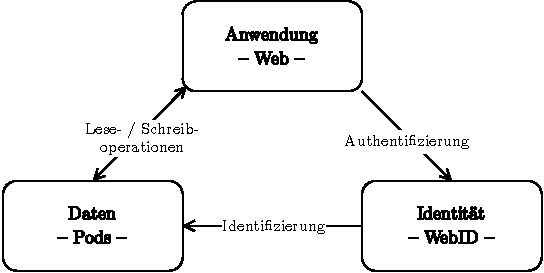
\includegraphics[width=0.7\textwidth]{./assets/solid_triangle.drawio.pdf}
    \caption{Komponenten von Solid}
    \label{fig:solid-components}
\end{figure}


\subsection{Datenmanagement und Datenzugriff}

Daten werden, entsprechend des Data Space Konzepts, dezentral in sog. \emph{Personal Online Data Stores} (Pods) und nicht zentral bei den Anwendungen gespeichert~\cite{mecklerWebLinkedData2023}.
% Datenstruktur
Da Binärdateien schlecht maschinell lesbar und somit schlecht automatisiert verarbeitbar sind, müssen zusätzliche Metadaten gespeichert werden.
Ein lesbares Format für Mensch und Maschine ist jedoch anzustreben, um eine Automatisierung zu ermöglichen.
Dafür wird das \emph{Resource Description Framework} (RDF) verwendet, welches Daten als Subjekt"=Prädikat"=Objekt"=Tripel speichert (vgl. Semantic Web).
Für die Strukturierung und Speicherung von Semantik werden \emph{Vocabularies} verwendet.
In Kombination mit einer Verknüpfung nach dem Ansatz von \emph{Linked Data} entstehen automatisierbare, semantische Daten, welche mit verwandten Ressourcen vernetzt sind~\cite{bizerLinkedDataStory2009,mecklerWebLinkedData2023,sambraSolidPlatformDecentralized2016}.
Andere Datenstrukturen können mittels Mapping zu RDF oder als Binärdateien mit zusätzlichen Metadaten zur Speicherung der Semantik in Pods integriert werden~\cite{mecklerWebLinkedData2023,sambraSolidPlatformDecentralized2016}.

Organisiert werden die Daten in \emph{LDP"=Containern}, welche vergleichbar mit einem Verzeichnis sind.
Diese sind an sich selbst ein RDF"=Graph, wodurch eine Hierarchie durch Verschachtelung möglich ist.
Auf jeder Ebene der Hierarchie kann eine Zugriffskontrolle über \emph{Access Control List} Ressourcen definiert werden.
Es können unterschiedliche Rechte pro Akteur sowie pro Ressource bzw. Container eingerichtet werden.

% Lesen und Schreiben
Solid"=Anwendungen lesen und schreiben Daten direkt von und in den Pods.
Da Pods interoperabel mit den Anwendungen sein müssen, um eine Austauschbarkeit zu gewährleisten, muss ein wohldefiniertes und möglich einfach implementierbares Protokoll zum Datenzugriff verwendet werden.
Solid verwendet dabei RESTful"=Methoden basierend auf der \emph{Linked Data Platform} (LDP).
Diese definiert bestimmte HTTP"=Operationen auf Web"=Ressourcen, wodurch alle CRUD"=Operationen abgedeckt werden.
Um eine Ressource eindeutig zu identifizieren, ist jeder Ressource ein \emph{Uniform Resource Identifier} (URI) zugewiesen~\cite{mecklerWebLinkedData2023,sambraSolidPlatformDecentralized2016}.

% SPARQL
Mit den LDP"=Methoden sind jedoch nur einfache Anfragen möglich.
Komplizierte Datenabfragen können optional mittels SPARQL unterstützt werden.
Um den Entwicklungsaufwand zu verringern, werden diese Operationen an den Server delegiert.
Dabei sind \emph{Local Queries}, welche nur innerhalb \emph{eines} Pods operieren, und \emph{Link Following Queries}, welche über mehrere Pods hinweg mittels Verfolgung von Links operieren, möglich.
Die tatsächliche Verteilung muss dabei nicht bekannt sein~\cite{sambraSolidPlatformDecentralized2016}.

\textcolor{red}{TODO: Zusammenfassung, Ziele}


\subsection{Identität und Authentifizierung}
